\documentclass[a4paper]{article} 
\usepackage{amsmath,amsfonts,bm}
\usepackage{hyperref}
\usepackage{amsthm} 
\usepackage{geometry}
\usepackage{amssymb}
\usepackage{pstricks-add}
\usepackage{framed,mdframed}
\usepackage{graphicx,color} 
\usepackage{mathrsfs,xcolor} 
\usepackage[all]{xy}
\usepackage{fancybox} 
% \usepackage{CJKutf8}
\usepackage{xeCJK}
\newtheorem{theorem}{定理}
\newtheorem{lemma}{引理}
\newtheorem{corollary}{推论}
\newtheorem*{exercise}{习题}
\newtheorem{example}{例}
\geometry{left=2.5cm,right=2.5cm,top=2.5cm,bottom=2.5cm}
\setCJKmainfont[BoldFont=Adobe Heiti Std R]{Adobe Song Std L}
\renewcommand{\today}{\number\year 年 \number\month 月 \number\day 日}
\newcommand{\D}{\displaystyle}
\newcommand{\ds}{\displaystyle} \renewcommand{\ni}{\noindent}
\newcommand{\pa}{\partial} \newcommand{\Om}{\Omega}
\newcommand{\om}{\omega} \newcommand{\sik}{\sum_{i=1}^k}
\newcommand{\vov}{\Vert\omega\Vert} \newcommand{\Umy}{U_{\mu_i,y^i}}
\newcommand{\lamns}{\lambda_n^{^{\scriptstyle\sigma}}}
\newcommand{\chiomn}{\chi_{_{\Omega_n}}}
\newcommand{\ullim}{\underline{\lim}} \newcommand{\bsy}{\boldsymbol}
\newcommand{\mvb}{\mathversion{bold}} \newcommand{\la}{\lambda}
\newcommand{\La}{\Lambda} \newcommand{\va}{\varepsilon}
\newcommand{\be}{\beta} \newcommand{\al}{\alpha}
\newcommand{\dis}{\displaystyle} \newcommand{\R}{{\mathbb R}}
\newcommand{\N}{{\mathbb N}} \newcommand{\cF}{{\mathcal F}}
\newcommand{\gB}{{\mathfrak B}} \newcommand{\eps}{\epsilon}
\renewcommand\refname{参考文献}
\begin{document}
\title{\huge{\bf{利用几何变换的观点解一道平面几何题}}} \author{\small{叶卢
    庆\footnote{叶卢庆(1992---),男,杭州师范大学理学院数学与应用数学专业
      本科在读,E-mail:h5411167@gmail.com}}\\{\small{杭州师范大学理学院,浙
      江~杭州~310036}}}
\maketitle
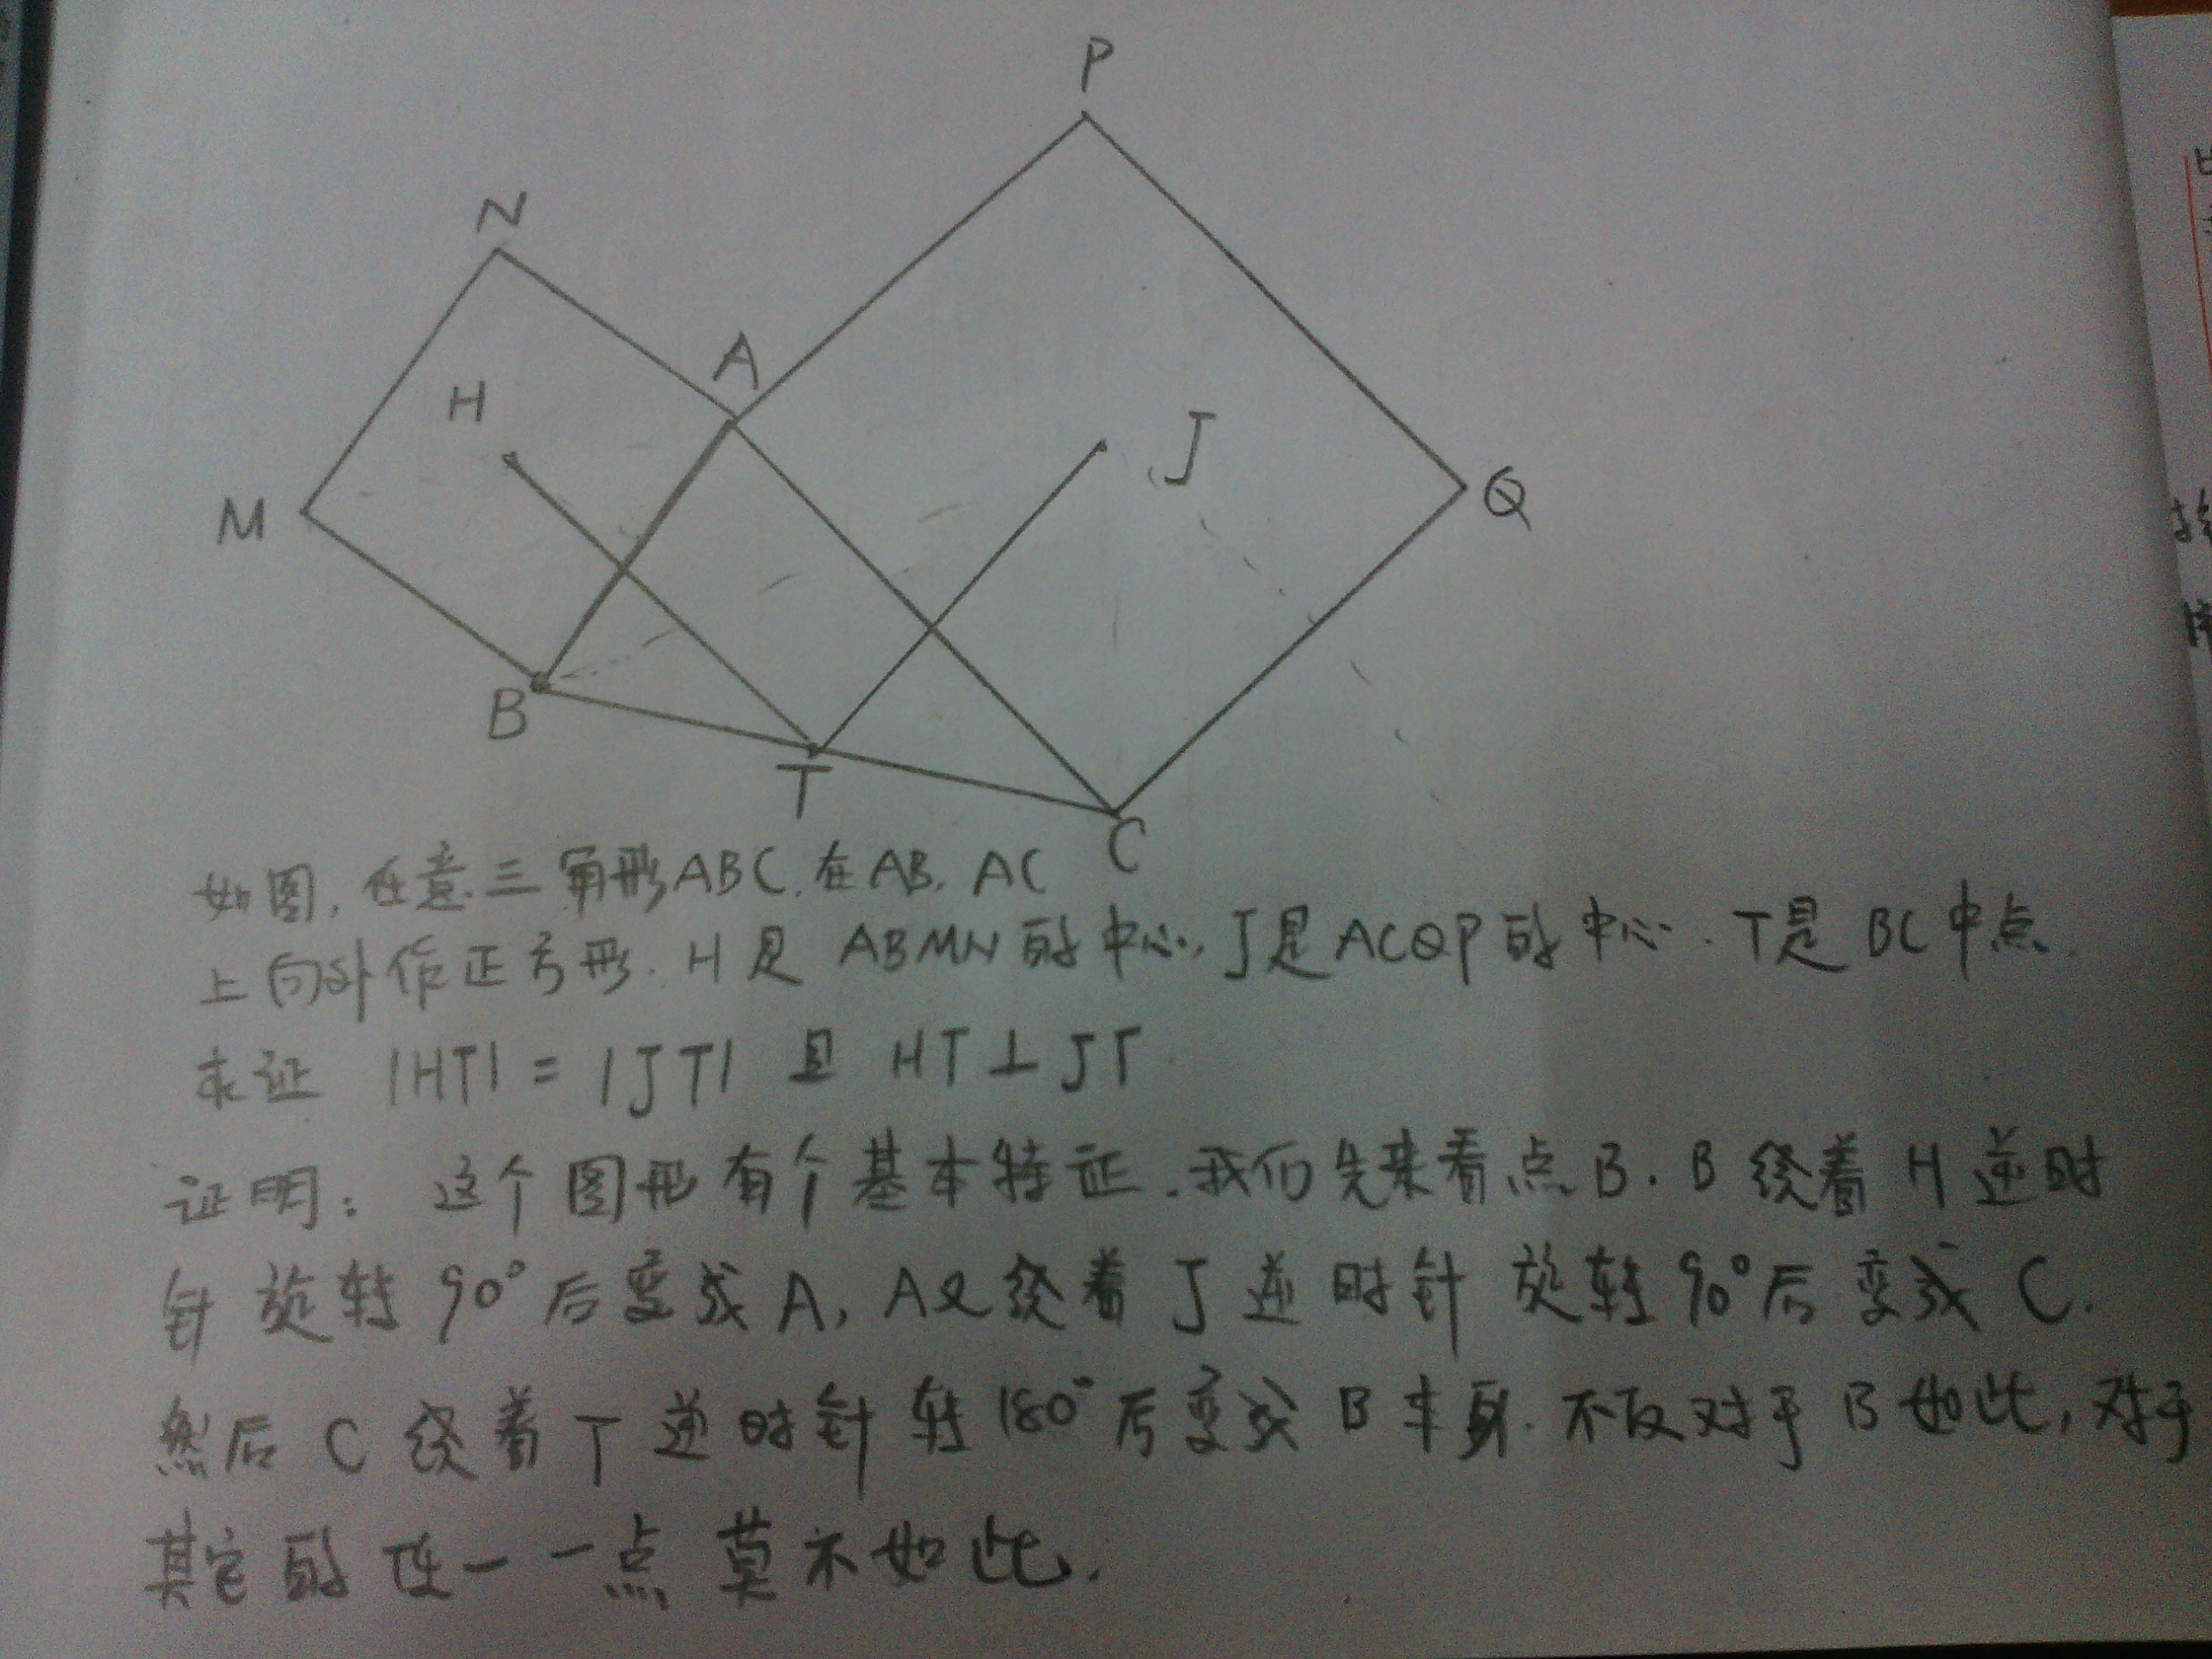
\includegraphics[width=1\textwidth]{/home/luqing/math/visual-complex-analysis/page17-2-1}
\newrgbcolor{zzttqq}{0.6 0.2 0}
\newrgbcolor{xdxdff}{0.49 0.49 1}
\psset{xunit=1.0cm,yunit=1.0cm,algebraic=true,dotstyle=o,dotsize=3pt 0,linewidth=0.8pt,arrowsize=3pt 2,arrowinset=0.25}
\begin{pspicture*}(2.34,-6.37)(26.78,6.86)
\pspolygon[linecolor=zzttqq,fillcolor=zzttqq,fillstyle=solid,opacity=0.1](11.28,2.26)(8.62,-1.32)(13.08,-1.76)
\pspolygon[linecolor=zzttqq,fillcolor=zzttqq,fillstyle=solid,opacity=0.1](11.28,2.26)(13.08,-1.76)(17.1,0.04)(15.3,4.06)
\pspolygon[linecolor=zzttqq,fillcolor=zzttqq,fillstyle=solid,opacity=0.1](8.62,-1.32)(11.28,2.26)(7.7,4.92)(5.04,1.34)
\psline[linecolor=zzttqq](11.28,2.26)(8.62,-1.32)
\psline[linecolor=zzttqq](8.62,-1.32)(13.08,-1.76)
\psline[linecolor=zzttqq](13.08,-1.76)(11.28,2.26)
\psline[linecolor=zzttqq](11.28,2.26)(13.08,-1.76)
\psline[linecolor=zzttqq](13.08,-1.76)(17.1,0.04)
\psline[linecolor=zzttqq](17.1,0.04)(15.3,4.06)
\psline[linecolor=zzttqq](15.3,4.06)(11.28,2.26)
\psline[linecolor=zzttqq](8.62,-1.32)(11.28,2.26)
\psline[linecolor=zzttqq](11.28,2.26)(7.7,4.92)
\psline[linecolor=zzttqq](7.7,4.92)(5.04,1.34)
\psline[linecolor=zzttqq](5.04,1.34)(8.62,-1.32)
\psline(8.62,-1.32)(14.19,1.15)
\psline(14.19,1.15)(16.61,-4.44)
\psline(5.04,1.34)(16.61,-4.44)
\begin{scriptsize}
\psdots[dotstyle=*,linecolor=blue](11.28,2.26)
\rput[bl](11.38,2.39){\blue{$A$}}
\psdots[dotstyle=*,linecolor=blue](8.62,-1.32)
\rput[bl](8.71,-1.17){\blue{$B$}}
\psdots[dotstyle=*,linecolor=blue](13.08,-1.76)
\rput[bl](13.18,-1.63){\blue{$C$}}
\psdots[dotstyle=*,linecolor=darkgray](17.1,0.04)
\rput[bl](17.19,0.17){\darkgray{$Q$}}
\psdots[dotstyle=*,linecolor=darkgray](15.3,4.06)
\rput[bl](15.39,4.19){\darkgray{$P$}}
\psdots[dotstyle=*,linecolor=darkgray](7.7,4.92)
\rput[bl](7.8,5.05){\darkgray{$N$}}
\psdots[dotstyle=*,linecolor=darkgray](5.04,1.34)
\rput[bl](5.13,1.47){\darkgray{$M$}}
\psdots[dotstyle=*,linecolor=darkgray](10.85,-1.54)
\rput[bl](10.94,-1.4){\darkgray{$T$}}
\psdots[dotstyle=*,linecolor=darkgray](8.16,1.8)
\rput[bl](8.25,1.93){\darkgray{$H$}}
\psdots[dotstyle=*,linecolor=darkgray](14.19,1.15)
\rput[bl](14.27,1.29){\darkgray{$J$}}
\psdots[dotstyle=*,linecolor=xdxdff](16.61,-4.44)
\rput[bl](16.69,-4.3){\xdxdff{$E$}}
\end{scriptsize}
\end{pspicture*}
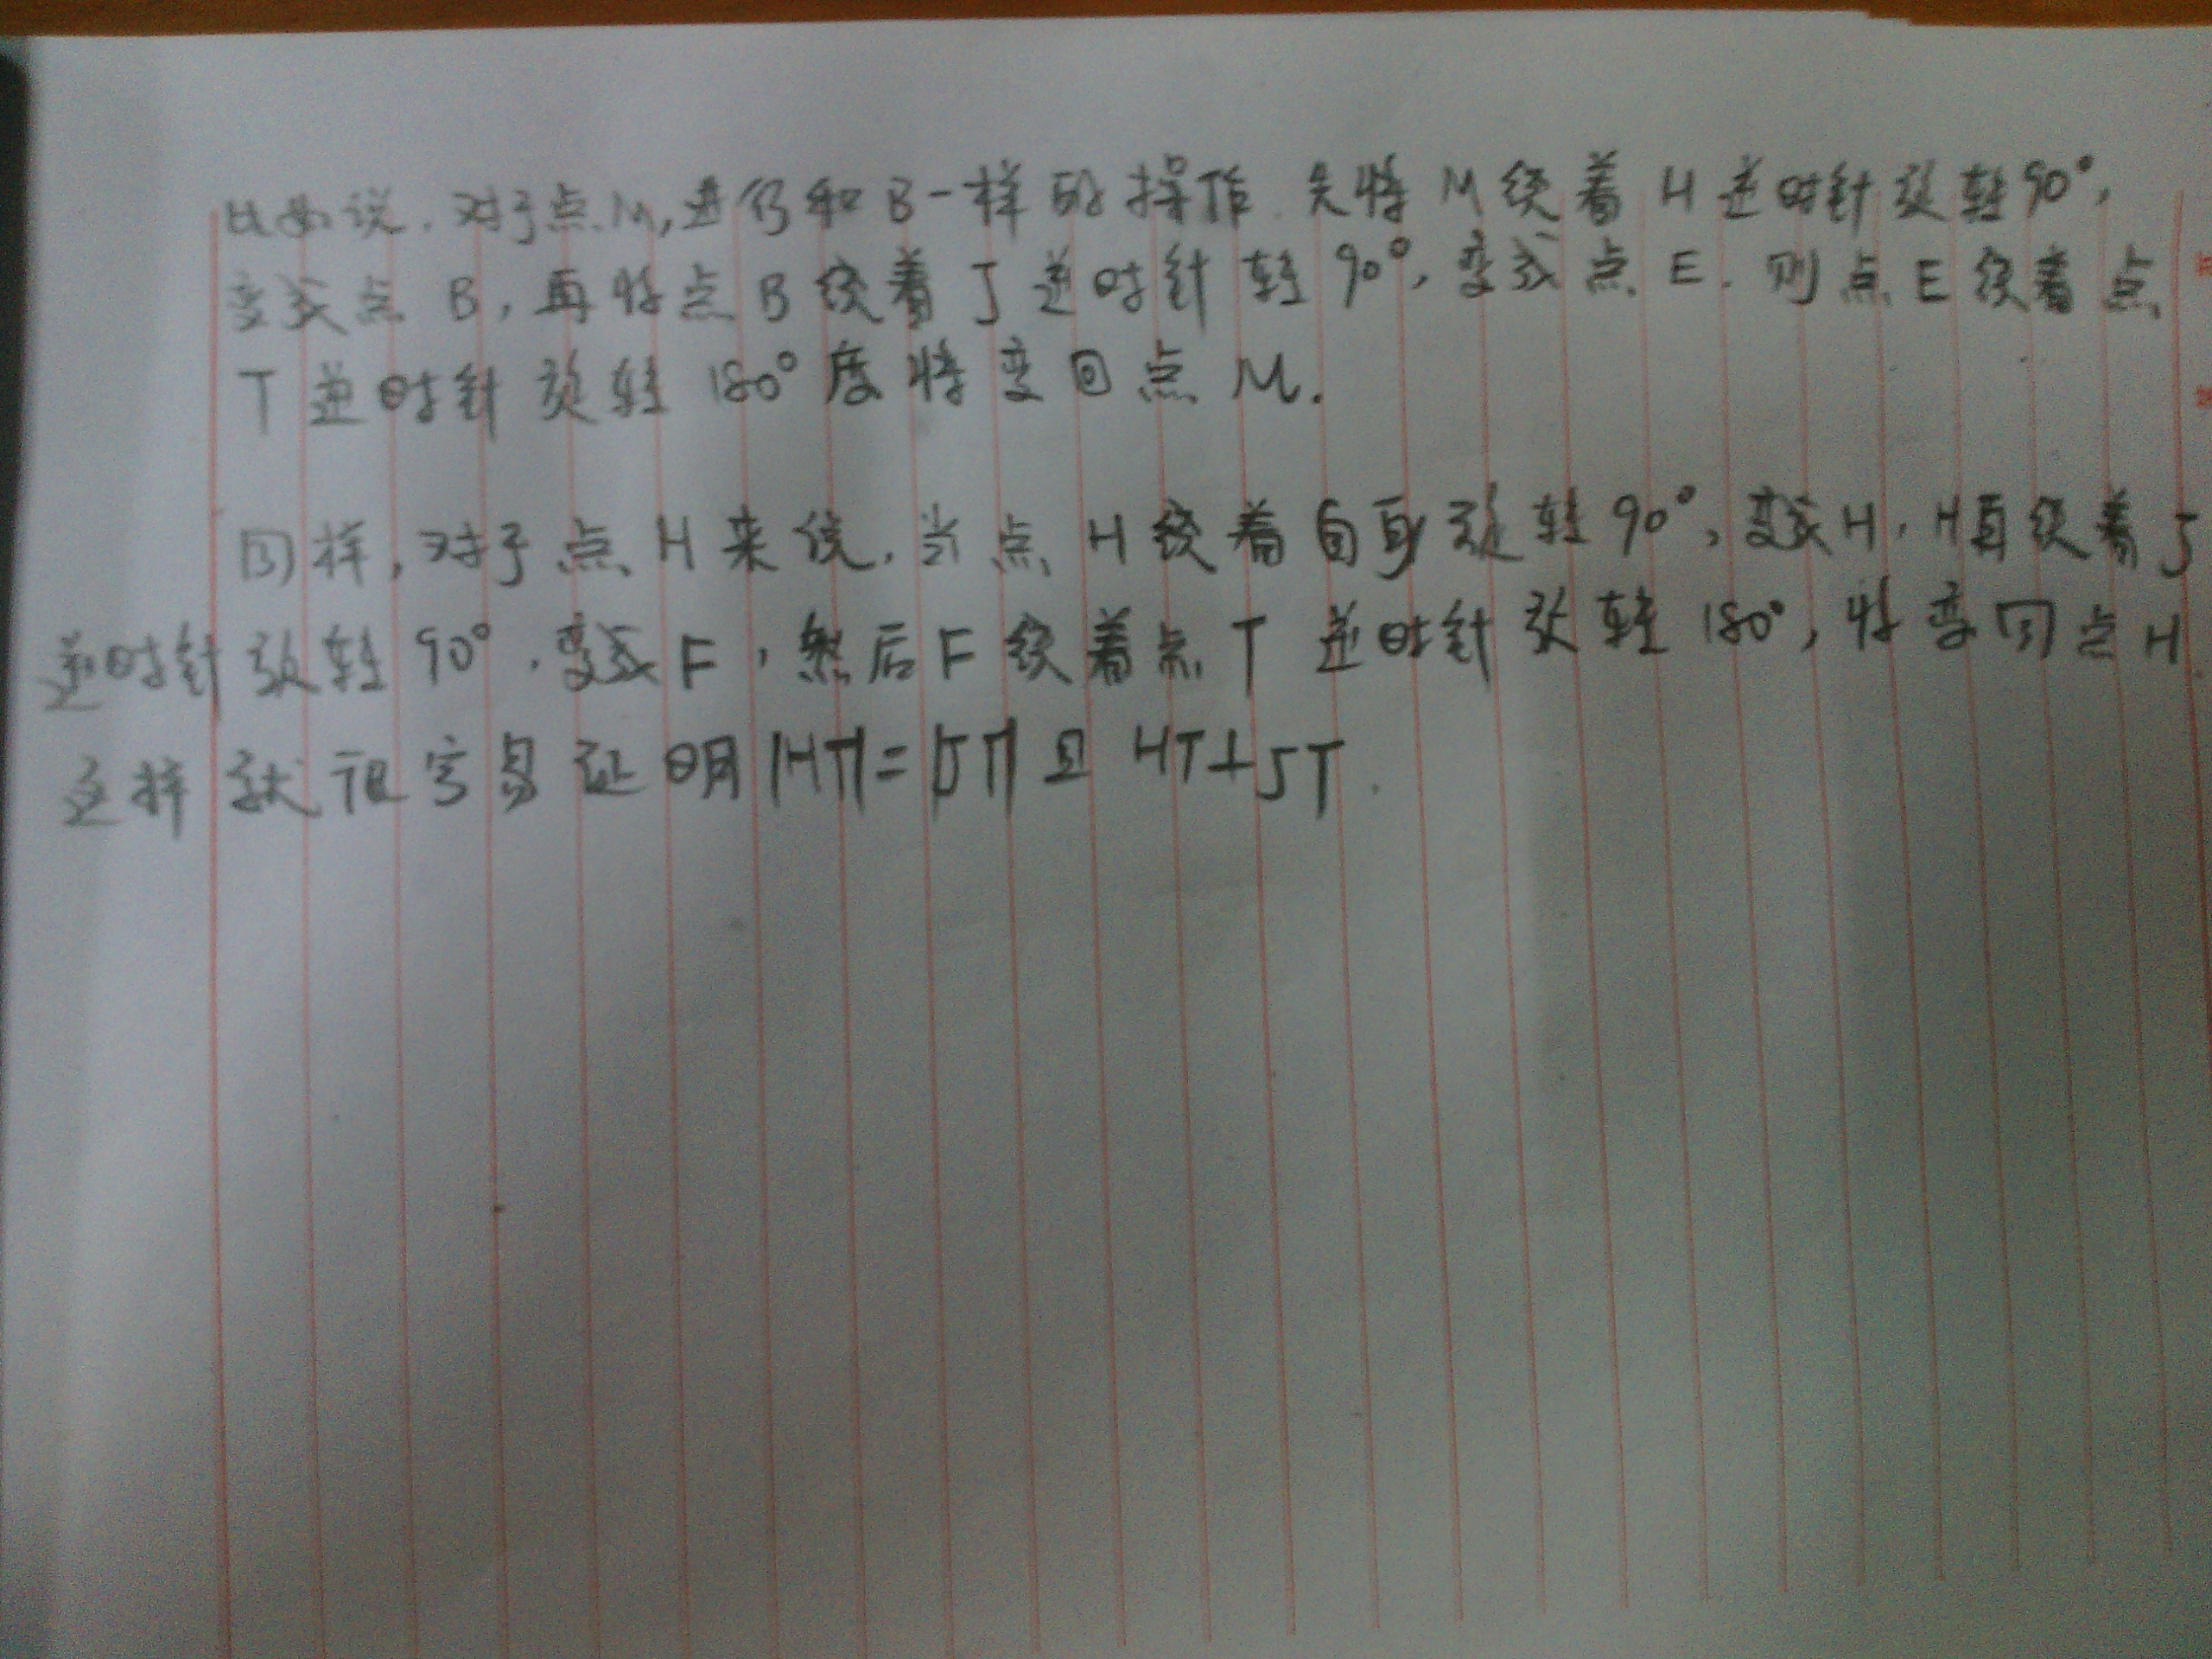
\includegraphics[width=1\textwidth]{/home/luqing/math/visual-complex-analysis/IMG20140224184016.jpg}
\newcommand{\degre}{\ensuremath{^\circ}}
\newrgbcolor{zzttqq}{0.6 0.2 0}
\newrgbcolor{qqwuqq}{0 0.39 0}
\psset{xunit=1.0cm,yunit=1.0cm,algebraic=true,dotstyle=o,dotsize=3pt 0,linewidth=0.8pt,arrowsize=3pt 2,arrowinset=0.25}
\begin{pspicture*}(2.34,-7.04)(26.82,6.86)
\pspolygon[linecolor=zzttqq,fillcolor=zzttqq,fillstyle=solid,opacity=0.1](11.28,2.26)(8.62,-1.32)(13.08,-1.76)
\pspolygon[linecolor=zzttqq,fillcolor=zzttqq,fillstyle=solid,opacity=0.1](11.28,2.26)(13.08,-1.76)(17.1,0.04)(15.3,4.06)
\pspolygon[linecolor=zzttqq,fillcolor=zzttqq,fillstyle=solid,opacity=0.1](8.62,-1.32)(11.28,2.26)(7.7,4.92)(5.04,1.34)
\pspolygon[linecolor=qqwuqq,fillcolor=qqwuqq,fillstyle=solid,opacity=0.1](13.71,1.2)(13.66,0.72)(14.14,0.67)(14.19,1.15)
\psline[linecolor=zzttqq](11.28,2.26)(8.62,-1.32)
\psline[linecolor=zzttqq](8.62,-1.32)(13.08,-1.76)
\psline[linecolor=zzttqq](13.08,-1.76)(11.28,2.26)
\psline[linecolor=zzttqq](11.28,2.26)(13.08,-1.76)
\psline[linecolor=zzttqq](13.08,-1.76)(17.1,0.04)
\psline[linecolor=zzttqq](17.1,0.04)(15.3,4.06)
\psline[linecolor=zzttqq](15.3,4.06)(11.28,2.26)
\psline[linecolor=zzttqq](8.62,-1.32)(11.28,2.26)
\psline[linecolor=zzttqq](11.28,2.26)(7.7,4.92)
\psline[linecolor=zzttqq](7.7,4.92)(5.04,1.34)
\psline[linecolor=zzttqq](5.04,1.34)(8.62,-1.32)
\psline(8.16,1.8)(10.85,-1.54)
\psline(10.85,-1.54)(14.19,1.15)
\psline(10.85,-1.54)(13.54,-4.88)
\psline(8.16,1.8)(14.19,1.15)
\psline(14.19,1.15)(13.54,-4.88)
\pscustom[linecolor=qqwuqq,fillcolor=qqwuqq,fillstyle=solid,opacity=0.1]{\parametricplot{2.2488147518204507}{5.390407405410244}{0.68*cos(t)+10.85|0.68*sin(t)+-1.54}\lineto(10.85,-1.54)\closepath}
\begin{scriptsize}
\psdots[dotstyle=*,linecolor=blue](11.28,2.26)
\rput[bl](11.38,2.39){\blue{$A$}}
\psdots[dotstyle=*,linecolor=blue](8.62,-1.32)
\rput[bl](8.71,-1.17){\blue{$B$}}
\psdots[dotstyle=*,linecolor=blue](13.08,-1.76)
\rput[bl](13.18,-1.63){\blue{$C$}}
\psdots[dotstyle=*,linecolor=darkgray](17.1,0.04)
\rput[bl](17.19,0.17){\darkgray{$Q$}}
\psdots[dotstyle=*,linecolor=darkgray](15.3,4.06)
\rput[bl](15.39,4.19){\darkgray{$P$}}
\psdots[dotstyle=*,linecolor=darkgray](7.7,4.92)
\rput[bl](7.8,5.05){\darkgray{$N$}}
\psdots[dotstyle=*,linecolor=darkgray](5.04,1.34)
\rput[bl](5.13,1.47){\darkgray{$M$}}
\psdots[dotstyle=*,linecolor=darkgray](10.85,-1.54)
\rput[bl](10.94,-1.4){\darkgray{$T$}}
\psdots[dotstyle=*,linecolor=darkgray](8.16,1.8)
\rput[bl](8.25,1.93){\darkgray{$H$}}
\psdots[dotstyle=*,linecolor=darkgray](14.19,1.15)
\rput[bl](14.27,1.29){\darkgray{$J$}}
\psdots[dotstyle=*,linecolor=darkgray](13.54,-4.88)
\rput[bl](13.64,-4.73){\darkgray{$F$}}
\psdots[dotstyle=*,linecolor=darkgray](13.54,-4.88)
\rput[bl](13.64,-4.73){\darkgray{$H'$}}
\rput[bl](13.8,0.79){\qqwuqq{$90\textrm{\degre}$}}
\psdots[dotstyle=*,linecolor=darkgray](13.54,-4.88)
\rput[bl](13.64,-4.73){\darkgray{$H'_1$}}
\rput[bl](10.46,-1.9){\qqwuqq{$180\textrm{\degre}$}}
\end{scriptsize}
\end{pspicture*}
\end{document}








